\chapter{Der Photoeffekt}
\section{Grundlagen}
\subsection{Photoeffekt}
Der Photoeffekt tritt bei Ionisierung von Atomen durch Lichteinstrahlung, wobei die Energie der Valenzelektronen so weit ansteigt, dass sie das Potential des Atoms verlassen können. Dies geschieht nur, wenn das Licht eine Mindestenergie erreicht, die der Tiefe des Elektronenpotentials entspricht. Die Energie des Lichts \(E\) hängt mit ihrer Frequenz \(\nu\) durch die Beziehung \(E = \nu h\) zusammen, wobei \(h\) das Plancksche Wirkungsquantum darstellt. 
\subsection{Funktionsweise einer Photozelle}
\paragraph{Aufbau}
Eine Photozelle besteht aus einer Ringanode und einer Kathode, welche mit Licht beleuchtet
wird. Die Anode und die Kathode bestehen aus unterschiedlichen Materialien.


\begin{figure}[htbp]
    \centering
    \includegraphics[width=0.75\textwidth]{figs/anlegen_aeuß_potential.png}
    \caption{ Kontaktpotential $-eU_{KA}$ \cite{praktikum}}
    \label{fig:potential ext}
\end{figure}
\FloatBarrier

\begin{figure}[htbp]
    \centering
    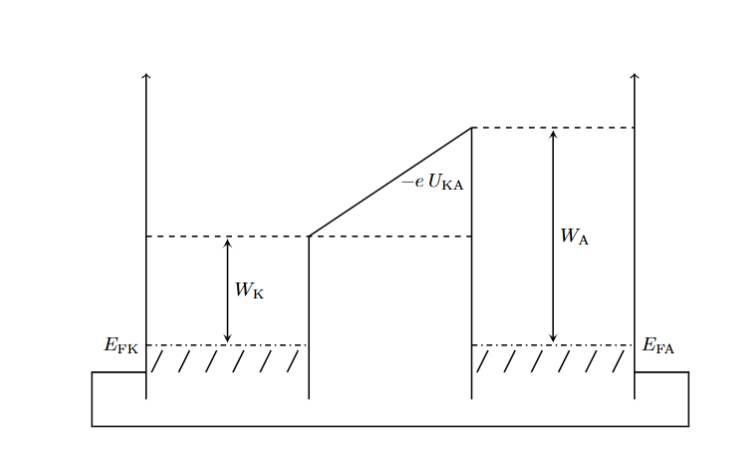
\includegraphics[width=0.75\textwidth]{figs/kontaktpotential_kurzgeschl_elektroden.png}
    \caption{  Potential dass von der Gegenspannung
$-eU_G$ induziert wird\cite{praktikum}}
    \label{fig:potential kurzg.}
\end{figure}
\FloatBarrier

\paragraph{Wirkung}
\begin{figure}[htbp]
    \centering
    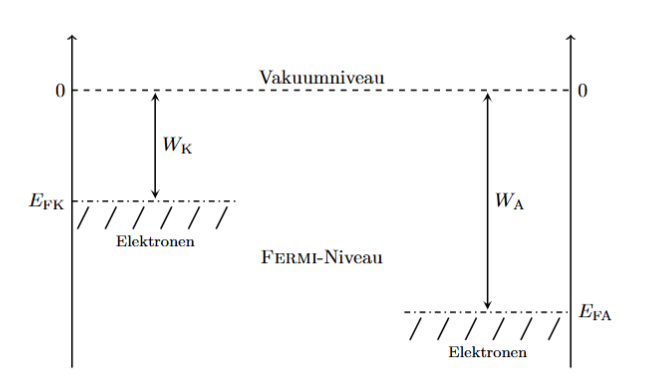
\includegraphics[width=0.75\textwidth]{figs/baenderschema_kathode_anode.png}
    \caption{ Ferminiveaus von Kathode und Anode mit Austrittsarbeit $W_A$ \cite{praktikum}}
    \label{fig:kathode-anode}
\end{figure}
\FloatBarrier
Das Anodenmaterial weist eine höhere Austrittsarbeit auf als das Kathodenmaterial, wodurch beim Kontakt eine Potentialdifferenz zwischen ihren Ferminiveaus entsteht. Diese Differenz verstärkt sich, wenn eine zusätzliche Gegenspannung zwischen Anode und Kathode angelegt wird.\\
Die durch das Licht herausgelösten Elektronen gewinnen entsprechend seiner Energie kinetische Energie und bewegen sich zur Anode, wodurch ein messbarer Strom entsteht. Die angelegte Gegenspannung verlangsamt die Elektronen und wird schrittweise erhöht, bis kein Photostrom mehr nachweisbar ist – also die Elektronen aus dem Anodenmaterial nicht mehr die Anode erreichen.
%\paragraph{Photostromverlauf}
%\paragraph{Austrittsarbeit}
%\paragraph{Kontaktpotential}

\section{Aufbau}
\begin{figure}[htbp]
    \centering
    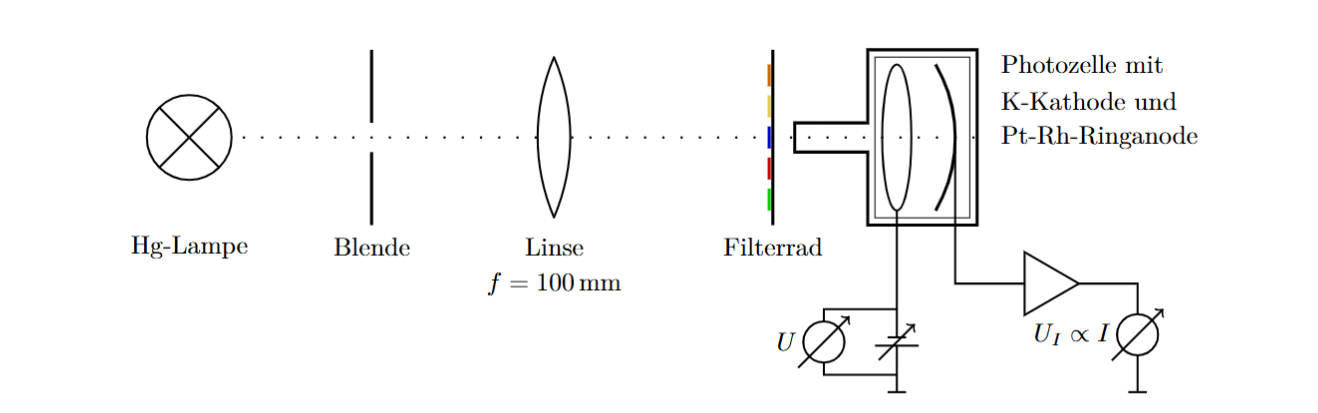
\includegraphics[width=0.75\textwidth]{figs/Aufbau_plank_wirkungsquantum.png}
    \caption{Aufbau für die Messung des Photoeffektes  \cite{praktikum}}
    \label{fig:aufbau teil 1}
\end{figure}
\FloatBarrier
Links ist die Hg-Lampe zu sehen, in der
Mitte Optik-Elemente zum Fokussieren und Filtern des Lichtes und rechts ist die Photozelle
mit Gegenspannung und Strommessung.

\section{Durchführung}
Die Quecksilber-Spektrallampe und die Photozelle werden gemäß Abbildung \ref{fig:aufbau teil 1} gegenüberliegend auf dem Reiter angeordnet. Eine Irisblende vor der Lampe ermöglicht die Regulierung der Lichtintensität. Eine Linse mit einer Brennweite von f=100 mm wird in diesem Abstand vor die Blende positioniert, sodass sie das Licht parallel auf den nachfolgenden Interferenzfilter mit fünf Filtern sowie eine zusätzliche Blende lenkt.\\
Eine Abschirmvorrichtung mit einem röhrenförmigen Element verhindert Streulicht. Ein Lichtfleck wird gezielt auf die Kathode projiziert, ohne ,dass die Anode beleuchtet wird. Der Anodenstrom wird über einen Messverstärker erfasst, während eine zum Strom proportionale Spannung mit einem Digitalmultimeter (DMM) gemessen wird. Die Gegenspannung stammt aus einem 12V-Gleichspannungsnetzteil, wobei der negative Pol mit der Anode verbunden ist, um die Elektronen abzubremsen. Diese Spannung wird mit einem weiteren DMM gemessen.
\subsection{Energiebilanz der Photoelektronen}
Laut der Abbildung der Ferminiveaus \ref{fig:kathode-anode} gilt für die Energiebilanz:
\begin{equation}
    E = h\nu = W_K + eU_{KA} + eU_{G,0} 
    = W_K + W_A - W_K + eU_{G,0} 
    = W_A + eU_{G,0}
\end{equation}\\
Aus der Frequenz des Lichtes können schließlich
die Austrittsarbeit der Anode $W_A$ und das Planck’sche Wirkungsquantum h bestimmt werden:
\begin{equation}
    eU_{G,0} = h\nu - W_A
\end{equation}
\section{Abschätzung des Plankschen Wirkungsquantum und der Austrittsarbeit}
\subsection{Bestimmung der Grenzspannung $U_0$}
\subsection{Bestimmung von Plankschen Wirkungsquantum $h$}
\subsection{Bestimmung der Austrittsarbeit $W_A$}
\subsection{Vergleich der $\lambda$ = Kennlinie für unterschiedliche Intensitäten }
%Diskussionen/Vergleiche werden direkt in den Unterteilen eingebaut
